\documentclass[a4paper]{article}

%% Language and font encodings
\usepackage[italian]{babel}
\usepackage[utf8x]{inputenc}
\usepackage[T1]{fontenc}

%% Sets page size and margins
\usepackage[a4paper,top=3cm,bottom=2cm,left=3cm,right=3cm,marginparwidth=1.75cm]{geometry}

%% Useful packages
\usepackage{graphicx}
\usepackage{float}
\usepackage[colorlinks=true, allcolors=blue]{hyperref}

\title{Quadrice}
\author{Girolamo Crocetti}

\begin{document}
\maketitle

\begin{figure}[H]
	\centering
	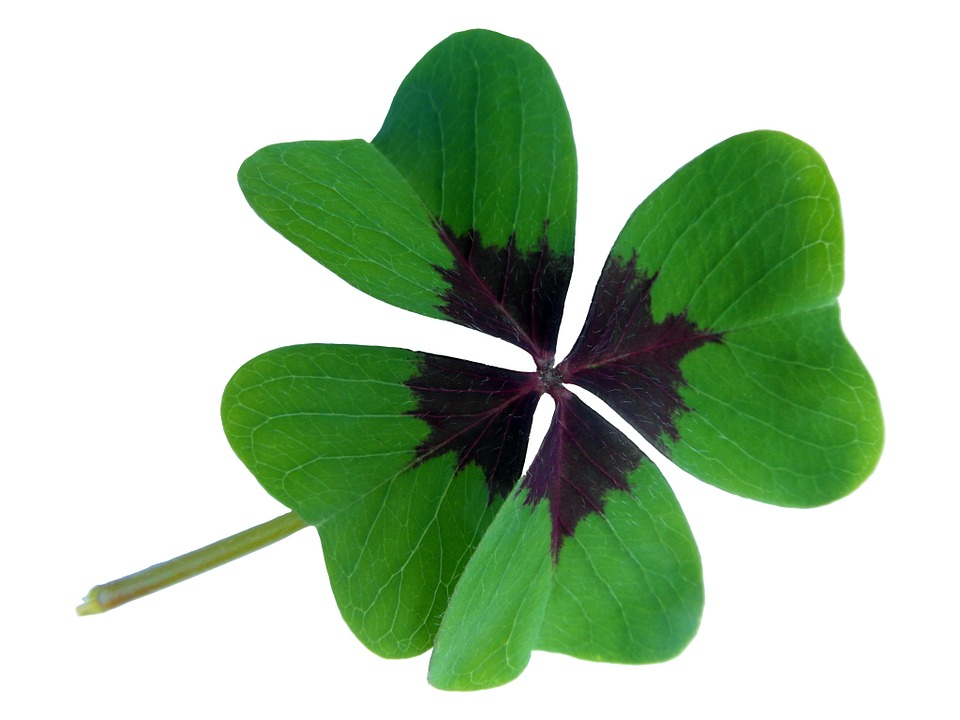
\includegraphics[width=0.3\linewidth]{Quadrice.jpg}
	\caption{Logo Quadrice}
\end{figure}

\section{Descrizione}

Quadrice permette di quadruplicare un numero intero.

\section{Operazioni}

Quadrice espone una sola operazione di segnatura quadrice( t1 )( int ).

\section{Tipi}

Il tipo t1 è la variante utilizzata da Quadrice del tipo di autenticazione di APIMarket.
\begin{itemize}
	\item t1: int;
	\item .key: string;
	\item .user: string;
	\item .api: int.
\end{itemize}

\end{document}